% =============================================================================
% LOATO-Bench: Evaluating Cross-Attack Generalization of Embedding-Based
% Prompt Injection Classifiers
% =============================================================================
\documentclass[conference]{IEEEtran}

% --- Packages ----------------------------------------------------------------
\usepackage{cite}
\usepackage{amsmath,amssymb}
\usepackage{graphicx}
\usepackage{booktabs}
\usepackage{multirow}
\usepackage{xcolor}
\usepackage{enumitem}
\usepackage{url}
\usepackage{microtype}
\usepackage{hyperref}

\hypersetup{
  colorlinks=true,
  linkcolor=blue!60!black,
  citecolor=blue!60!black,
  urlcolor=blue!60!black,
}

% --- Custom commands ---------------------------------------------------------
\newcommand{\df}{$\Delta$F1}
\newcommand{\Fone}{F1}

\title{LOATO-Bench: Evaluating Cross-Attack Generalization
       of Embedding-Based Prompt Injection Classifiers}

\author{
\IEEEauthorblockN{Ali Khan}
\IEEEauthorblockA{MS Data Science\\Pace University\\
  \texttt{ak58214n@pace.edu}}
\and
\IEEEauthorblockN{Ahmad Mukhtar}
\IEEEauthorblockA{MS Data Science\\Pace University\\
  \texttt{am41491n@pace.edu}}
}

\begin{document}
\maketitle

% =============================================================================
% ABSTRACT
% =============================================================================
\begin{abstract}
Embedding-based prompt injection classifiers achieve 0.977--0.997 \Fone{} under
standard cross-validation, suggesting deployment readiness. However, standard CV
guarantees every attack type appears in training---a condition violated when
novel techniques emerge. We introduce LOATO-Bench (Leave-One-Attack-Type-Out
Benchmark), an evaluation framework that holds out entire attack categories
during training. Using 68,845 samples from 9 public sources with a 7-category
attack taxonomy, we evaluate 5 embedding models $\times$ 4 classifiers under
three protocols: standard 5-fold CV, LOATO, and direct-to-indirect transfer.
LOATO reveals a mean generalization gap of \df{} = 0.051 across all 20
combinations (0.034 excluding SVM's kernel approximation), with
obfuscation/encoding attacks causing the largest drops (\Fone{} = 0.874 when
held out). More critically, classifiers scoring 0.997 \Fone{} under standard CV
collapse to 0.21--0.41 when tested on indirect injections unseen during
training. A GPT-4o zero-shot baseline achieves 0.71 \Fone{} on the same test
set---a +0.30 advantage requiring no training---confirming the failure is
architectural. Standard CV is insufficient for evaluating prompt injection
classifiers intended for production deployment.
\end{abstract}

\begin{IEEEkeywords}
prompt injection, adversarial attacks, embedding classifiers, evaluation
methodology, generalization, LLM security
\end{IEEEkeywords}

% =============================================================================
% 1. INTRODUCTION
% =============================================================================
\section{Introduction}
\label{sec:intro}

Large Language Models (LLMs) deployed in RAG pipelines, chatbots, and AI agents
are vulnerable to prompt injection attacks---malicious instructions embedded in
user inputs or retrieved documents that cause the model to deviate from its
intended behavior~\cite{perez2022ignore,greshake2023not}. A common defense is
an input-layer classifier that screens incoming text before it reaches the LLM.
These classifiers typically use sentence embeddings fed into a classical ML head
(logistic regression, XGBoost, MLP) and achieve \Fone{} scores exceeding 0.95
under standard evaluation.

The problem: standard evaluation (stratified $k$-fold cross-validation)
guarantees that every attack type appears in both training and test sets. This
does not reflect deployment reality, where attackers invent novel techniques the
classifier has never seen. A classifier that memorizes ``ignore previous
instructions'' will score perfectly on a test set containing that phrase, but
fail when the same intent is encoded in Base64 or embedded in a retrieved
document.

\textbf{Research question:} Can embedding-based prompt injection classifiers
generalize to novel attack types they have never seen during training?

\paragraph{Contributions.}
\begin{enumerate}[nosep,leftmargin=*]
\item \textbf{LOATO protocol}---a leave-one-attack-type-out evaluation
  framework that holds out entire attack categories, measuring generalization at
  the technique level (distinct from Fomin's~\cite{fomin2026benchmarks}
  dataset-level LODO).
\item \textbf{Direct-to-indirect transfer measurement}---the first controlled
  experiment showing \Fone{} collapse from 0.97 to 0.21--0.41 across 20
  embedding-classifier combinations.
\item \textbf{Unified benchmark dataset}---68,845 samples from 9 public sources
  with a 7-category taxonomy built via 3-tier labeling.
\item \textbf{LLM baseline contextualization}---GPT-4o zero-shot achieves +0.30
  \Fone{} on indirect injections at $\sim$800$\times$ higher cost, confirming
  the gap is architectural.
\end{enumerate}

Fig.~\ref{fig:elevator} summarizes the core finding: the best embedding
classifier collapses from 0.997 to 0.413 \Fone{} when the evaluation protocol
shifts from standard CV to direct-to-indirect transfer.

\begin{figure}[t]
  \centering
  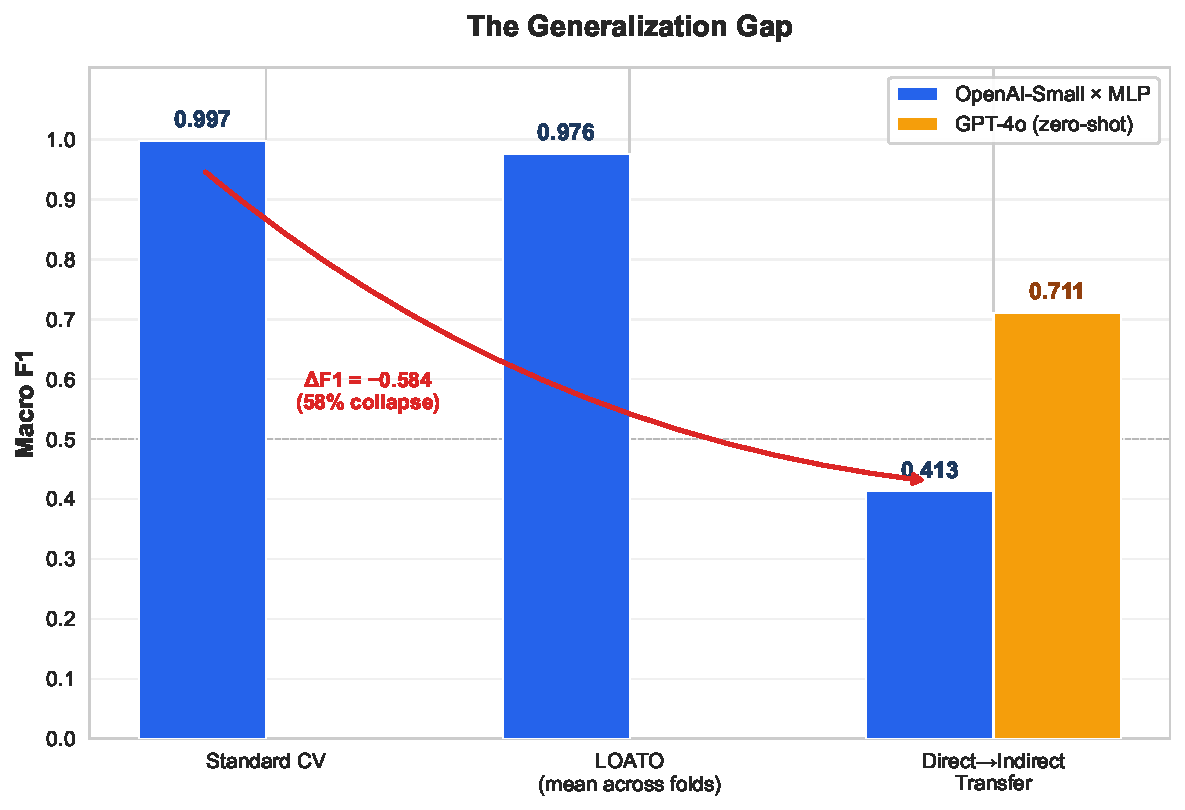
\includegraphics[width=0.95\columnwidth]{figures/generalization_gap_summary.pdf}
  \caption{The generalization gap. OpenAI-Small $\times$ MLP under three
    evaluation protocols, with GPT-4o zero-shot comparison on the transfer
    test. Standard CV dramatically overstates deployment safety.}
  \label{fig:elevator}
\end{figure}

% =============================================================================
% 2. RELATED WORK
% =============================================================================
\section{Related Work}
\label{sec:related}

\paragraph{Prompt injection attacks.}
Perez and Ribeiro~\cite{perez2022ignore} formalized direct prompt
injection---goal hijacking and prompt leaking via handcrafted adversarial
strings. Greshake et al.~\cite{greshake2023not} expanded the threat model
to \emph{indirect} injection, where malicious instructions are embedded in
retrieved documents rather than user inputs. Liu et
al.~\cite{liu2024formalizing} provided the first formal benchmarking
framework, evaluating 5 attack strategies and 10 defenses. Recent
surveys~\cite{esmradi2025comprehensive} catalogue the rapid evolution from
manual crafting to automated generation. The direct/indirect distinction is
central to our work: we show classifiers trained on direct injections collapse
when tested on indirect ones (Section~\ref{sec:transfer}).

\paragraph{Detection methods.}
Detection spans three paradigms: LLM-based guardrails
(LlamaGuard~\cite{inan2023llamaguard},
Prompt-Guard-2~\cite{meta2024promptguard},
Rebuff~\cite{protectai2023rebuff}), fine-tuned transformers
(Deepset's DeBERTa classifier~\cite{deepset2023promptinjections}), and
embedding-based classifiers with classical ML
heads~\cite{ayub2024embedding}. All three paradigms report performance on
in-distribution test sets. LOATO-Bench subjects the embedding+ML pattern to
out-of-distribution evaluation, revealing generalization failures that standard
reporting conceals.

\paragraph{Evaluation methodology.}
Li et al.~\cite{li2024oodrobustbench} demonstrated that adversarial
robustness degrades severely under distribution shift (OODRobustBench).
Fomin~\cite{fomin2026benchmarks} applied this insight to prompt
injection, proposing Leave-One-Dataset-Out (LODO) evaluation across 18 datasets
and revealing that standard splits inflate AUC by 8.4 percentage points.
LOATO-Bench is complementary: it holds out attack \emph{categories} within a
unified taxonomy rather than entire datasets, answering whether classifiers
generalize across technique boundaries rather than data sources.

\begin{table}[t]
\centering
\footnotesize
\caption{Comparison with Fomin~\cite{fomin2026benchmarks} (LODO).}
\label{tab:fomin}
\begin{tabular}{lll}
\toprule
\textbf{Dimension} & \textbf{LODO} & \textbf{LOATO (Ours)} \\
\midrule
Holdout unit & Entire dataset & Attack category \\
\# Datasets & 18 & 9 (unified + dedup) \\
Taxonomy & None & 7-category v1.0 \\
Detection approach & LLM activations & Embedding + ML \\
Direct$\to$indirect & 7--37\% (obs.) & 0.21--0.41 \Fone{} \\
Inflation finding & 8.4pp AUC & CV 0.97 $\to$ 0.21--0.41 \\
\bottomrule
\end{tabular}
\end{table}

% =============================================================================
% 3. DATASET
% =============================================================================
\section{Dataset}
\label{sec:dataset}

\subsection{Sources and Preprocessing}

We unified 9 public datasets---5 injection-focused
(Deepset~\cite{deepset2023promptinjections},
HackAPrompt~\cite{schulhoff2023hackaprompt},
GenTel-Bench~\cite{gentel2024bench},
PINT/Gandalf~\cite{lakera2023gandalf},
Open-Prompt-Injection~\cite{liu2024formalizing}) and 4 benign augmentation
sources (Dolly-15K, OASST1, WildChat, Alpaca). The preprocessing pipeline
applies NFC Unicode normalization, exact deduplication (SHA-256),
near-deduplication (MinHash LSH, Jaccard threshold 0.90, word 5-grams), and
language detection. GenTel-Bench~\cite{gentel2024bench} is a content-harm
dataset (not injection-specific); we repurposed its adversarial subset by
applying injection-confidence filtering via a 32-keyword heuristic scorer
(threshold 0.4), removing 71\% of non-injection samples.

The final dataset contains 68,845 samples: 40,003 benign (58.1\%) and 28,842
injection (41.9\%).

\subsection{Attack Taxonomy}

We developed a 7-category taxonomy via 3-tier labeling: (1) source-specific
mappings, (2) 32 regex patterns, and (3) GPT-4o-mini (temperature 0.0) for the
remaining $\sim$47\% of unmapped samples. When multiple strategies overlap, we
assign based on the dominant mechanism (e.g., an encoded jailbreak is C3, not
C2). Manual spot-check on 200 Tier-3 labels found 91\% agreement with the LLM
assignments; disagreements were concentrated at the C1/C7 boundary.

\begin{table}[t]
\centering
\footnotesize
\caption{Attack taxonomy (v1.0). C1--C5 are LOATO-eligible ($\geq$200
  samples). C6 has only 188 samples (a noted limitation).}
\label{tab:taxonomy}
\begin{tabular}{clrc}
\toprule
\textbf{ID} & \textbf{Category} & \textbf{N} & \textbf{LOATO} \\
\midrule
C1 & Instruction Override & 19,161 & \checkmark \\
C2 & Jailbreak / Roleplay & 1,614 & \checkmark \\
C3 & Obfuscation / Encoding & 545 & \checkmark \\
C4 & Information Extraction & 771 & \checkmark \\
C5 & Social Engineering & 311 & \checkmark \\
C6 & Context Manipulation & 188 & --- \\
C7 & Other / Multi-Strategy & 8,242 & --- \\
\bottomrule
\end{tabular}
\end{table}

\subsection{Template Homogeneity}
\label{sec:homogeneity}

Prompt injection datasets are highly templated. We quantify the degree to which
each held-out category's patterns are already represented in training via
\textbf{template homogeneity score}: the mean maximum cosine similarity between
each test sample's MiniLM embedding and its nearest training neighbor.

\begin{table}[t]
\centering
\footnotesize
\caption{Template homogeneity vs.\ generalization gap across all 6 LOATO
  folds. Higher homogeneity corresponds to lower \df{} ($r = -0.742$,
  $R^2 = 0.550$, $p = 0.092$, $n=6$).}
\label{tab:homogeneity}
\begin{tabular}{llcc}
\toprule
\textbf{ID} & \textbf{Category} & \textbf{Homog.} & \textbf{Mean \df{}} \\
\midrule
C1 & Instr.\ Override & 0.845 & 0.037 \\
C2 & Jailbreak / Roleplay & 0.676 & 0.049 \\
C3 & Obfusc.\ / Encoding & 0.670 & 0.090 \\
C4 & Info.\ Extraction & 0.675 & 0.051 \\
C5 & Social Engineering & 0.674 & 0.065 \\
C7 & Other / Multi-Strat.\ & 0.816 & 0.013 \\
\bottomrule
\end{tabular}
\end{table}

Fig.~\ref{fig:homogeneity} plots these 6 points: higher homogeneity predicts
lower \df{} ($r = -0.742$, $R^2 = 0.550$). C1 and C7 cluster at high
homogeneity / low gap; C3 is the outlier with lowest homogeneity and largest
gap. A UMAP projection (Fig.~\ref{fig:umap}) confirms that categories form
distinct clusters, with C1 spanning a broad, overlapping region.

\begin{figure}[t]
  \centering
  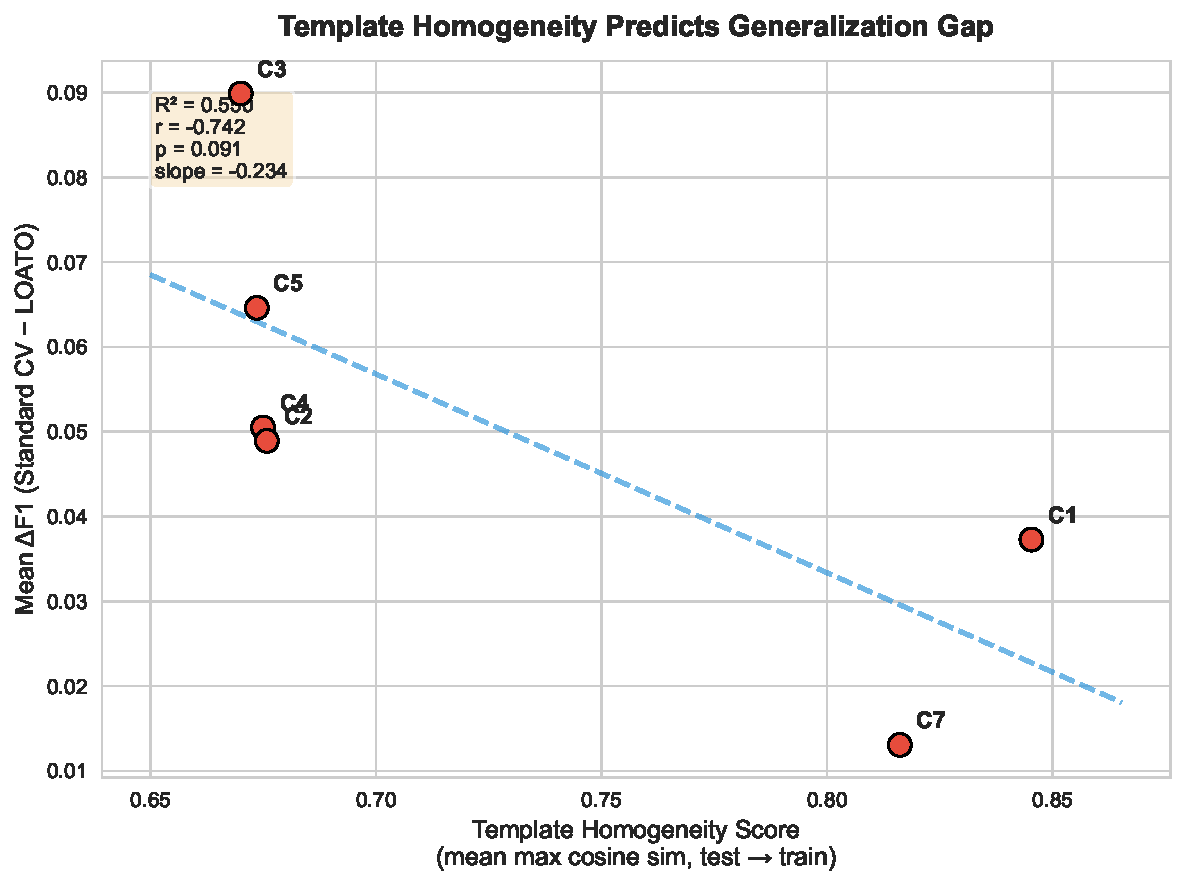
\includegraphics[width=0.95\columnwidth]{figures/homogeneity_vs_delta_f1.pdf}
  \caption{Template homogeneity vs.\ \df{} across 6 LOATO folds. Higher
    homogeneity (test samples resemble training) predicts smaller
    generalization gaps ($r = -0.742$, $R^2 = 0.550$).}
  \label{fig:homogeneity}
\end{figure}

\begin{figure}[t]
  \centering
  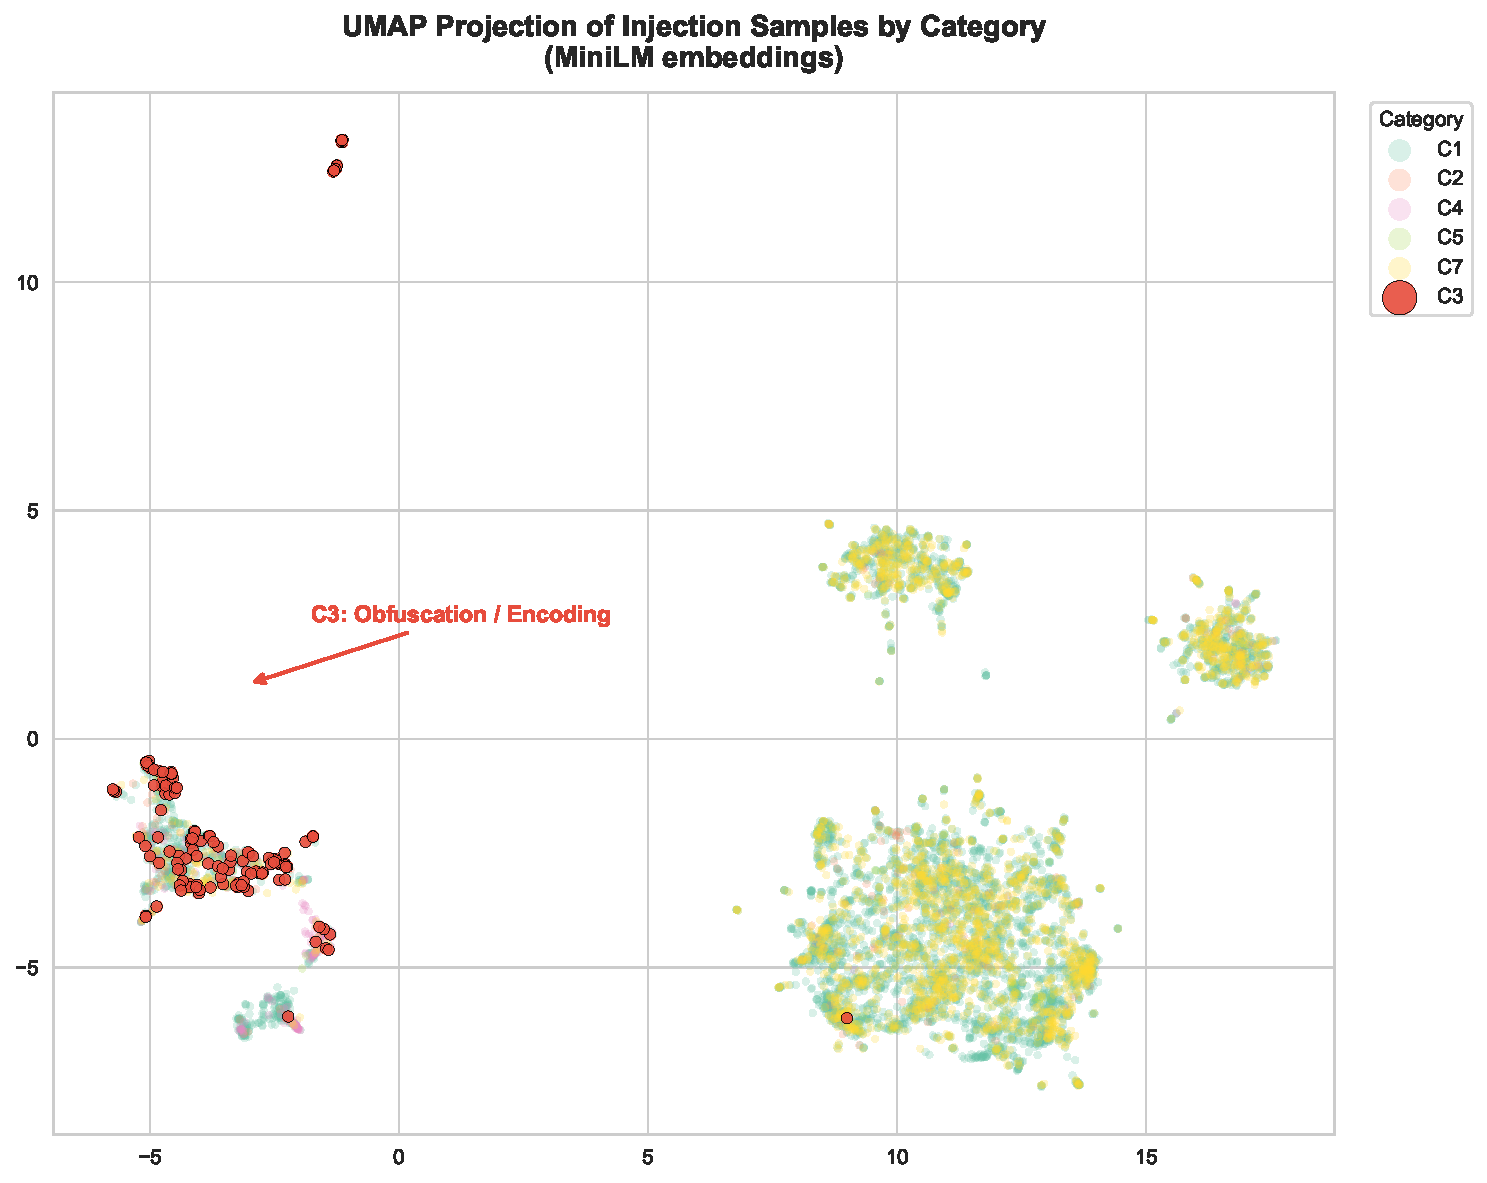
\includegraphics[width=0.95\columnwidth]{figures/umap_category_projection.pdf}
  \caption{UMAP projection of MiniLM embeddings colored by attack category,
    with C3 (Obfuscation / Encoding) highlighted in red. C1 (Instruction
    Override) overlaps broadly with other categories; C3 forms a distinct,
    isolated cluster---consistent with its largest generalization gap.}
  \label{fig:umap}
\end{figure}

% =============================================================================
% 4. METHODOLOGY
% =============================================================================
\section{Methodology}
\label{sec:method}

\subsection{Embedding Models}

We selected 5 models spanning 384--4096 dimensions, covering open-source and
proprietary, general-purpose and instruction-tuned (Table~\ref{tab:embeddings}).

\begin{table}[t]
\centering
\footnotesize
\caption{Embedding models evaluated.}
\label{tab:embeddings}
\begin{tabular}{lrl}
\toprule
\textbf{Model} & \textbf{Dim} & \textbf{Notes} \\
\midrule
all-MiniLM-L6-v2~\cite{reimers2019sentencebert} & 384 & Smallest \\
BGE-large-en-v1.5~\cite{xiao2023cpack} & 1024 & Prefix-cond.\ \\
Instructor-large~\cite{su2023instructor} & 768 & Instr.-tuned \\
text-emb-3-small~\cite{openai2024embeddings} & 1536 & OpenAI \\
E5-Mistral-7B~\cite{wang2024e5mistral} & 4096 & GGUF Q4 \\
\bottomrule
\end{tabular}
\end{table}

\subsection{Classifiers}

All classifiers use StandardScaler as a preprocessing step.
\textbf{Logistic Regression} ($C{=}1.0$, LBFGS),
\textbf{XGBoost} (300 trees, depth 6, lr 0.05),
\textbf{MLP} (256-128 hidden, early stopping), and
\textbf{SVM} (RBF kernel).
SVM uses Nystroem kernel approximation (500 components) with PCA(128) for
tractability on 68K samples---exact RBF-SVM is $O(n^2)$--$O(n^3)$ and
infeasible at this scale. SVM results should be interpreted as a lower bound;
this caveat applies wherever SVM numbers are reported.

\subsection{Evaluation Protocols}

\paragraph{Standard 5-Fold CV (baseline).}
Stratified on label and attack category. All attack types present in every fold.
Seed = 42.

\paragraph{LOATO (primary contribution).}
For each of the 5 eligible categories (C1--C5), the entire category is held out
from training. The test set includes the held-out category plus 20\% of benign
samples.

\paragraph{Direct$\to$Indirect Transfer.}
Train on direct injections only (5,930 samples from Deepset, HackAPrompt,
GenTel-Bench, PINT); test on indirect injections (22,898 samples from
Open-Prompt-Injection) plus 8,003 benign. No indirect samples appear during
training.

\paragraph{LLM Zero-Shot Baseline.}
GPT-4o evaluated with zero-shot binary classification on 500 stratified samples
per test pool. Temperature = 0. No few-shot examples.

\paragraph{Metrics.}
Primary: Macro \Fone{} (both classes weighted equally---critical for a 58/42\%
split where a majority-class baseline scores 58\% accuracy). Also: accuracy,
precision, recall, AUC-ROC.

\subsection{Reproducibility}
\label{sec:repro}

All experiments use seed 42. Hardware: Apple Silicon Mac (18~GB), MPS preferred.
The full pipeline is reproducible via CLI (Appendix~\ref{app:repro}). Code,
configs, and splits are version-controlled.\footnote{Code and data:
\url{https://github.com/alikhan126/loato-bench}}
Experiment tracking via Weights \& Biases.

% =============================================================================
% 5. RESULTS
% =============================================================================
\section{Results}
\label{sec:results}

\subsection{Standard CV: Classifiers Score 0.977--0.997 \Fone{}}

Under standard 5-fold CV, all 20 combinations achieve strong performance
(Table~\ref{tab:cv-compact}). Mean \Fone{} = 0.964; excluding SVM (kernel
approximation\footnote{SVM uses Nystroem(500) + PCA(128) approximation
throughout; see Section~\ref{sec:method}.}), the top 15 average 0.991. Best:
OpenAI-Small $\times$ MLP (0.997). These numbers look deployment-ready.

\begin{table}[t]
\centering
\footnotesize
\caption{Standard 5-fold CV: Macro \Fone{} (all 20 combinations). SVM$^*$
  uses Nystroem approximation.}
\label{tab:cv-compact}
\begin{tabular}{lcccc}
\toprule
\textbf{Embedding} & \textbf{LR} & \textbf{SVM$^*$} & \textbf{XGB} & \textbf{MLP} \\
\midrule
MiniLM       & .977 & .928 & .983 & .992 \\
BGE-Large    & .989 & .830 & .986 & .994 \\
Instructor   & .995 & .896 & .994 & .997 \\
OpenAI-Small & .995 & .902 & .993 & \textbf{.997} \\
E5-Mistral   & .994 & .851 & .987 & .996 \\
\bottomrule
\end{tabular}
\end{table}

\subsection{LOATO Reveals the Generalization Gap}
\label{sec:loato}

When a single attack category is held out, \Fone{} drops. Mean LOATO \Fone{}
across all 20 combinations: 0.913, yielding \df{} = 0.051. Excluding SVM, the
top 15 average 0.957 with \df{} = 0.034.

\begin{figure}[t]
  \centering
  
\includegraphics[width=0.95\columnwidth]{figures/delta_f1_heatmap.pdf}
  \caption{\df{} heatmap across embedding-classifier combinations. SVM
    (Nystroem approximation) shows the largest gaps; MLP the smallest.}
  \label{fig:heatmap}
\end{figure}

Key findings from Fig.~\ref{fig:heatmap}: (1) \textbf{Obfuscation/Encoding
(C3) is hardest}---mean \Fone{} = 0.874 when held out; SVM drops to 0.556.
(2) \textbf{MLP has the smallest gap} across all embeddings (0.018--0.029
\df{}). (3) \textbf{SVM has the largest gaps} (0.071--0.150 \df{}) due to the
Nystroem approximation limiting generalization. (4) Higher-quality embeddings
narrow the gap: MiniLM shows 0.029--0.118 \df{} range vs.\ Instructor/OpenAI at
0.019--0.047.

Statistical testing: 3/20 combinations show significant drops ($p < 0.05$,
paired $t$-test): MiniLM $\times$ LogReg, MiniLM $\times$ XGBoost, BGE-Large
$\times$ LogReg. With only 5--6 folds, most $p$-values fall in 0.06--0.15.

Fig.~\ref{fig:cm} shows confusion matrices for the best model (OpenAI-Small
$\times$ MLP) across all 6 LOATO folds, confirming the classifier does not
default to majority-class prediction. Even on the hardest fold (C3:
Obfuscation), the model achieves 0.925 \Fone{} with most errors concentrated
in false negatives (missed injections), not trivial majority-class assignment.

\begin{figure*}[t]
  \centering
  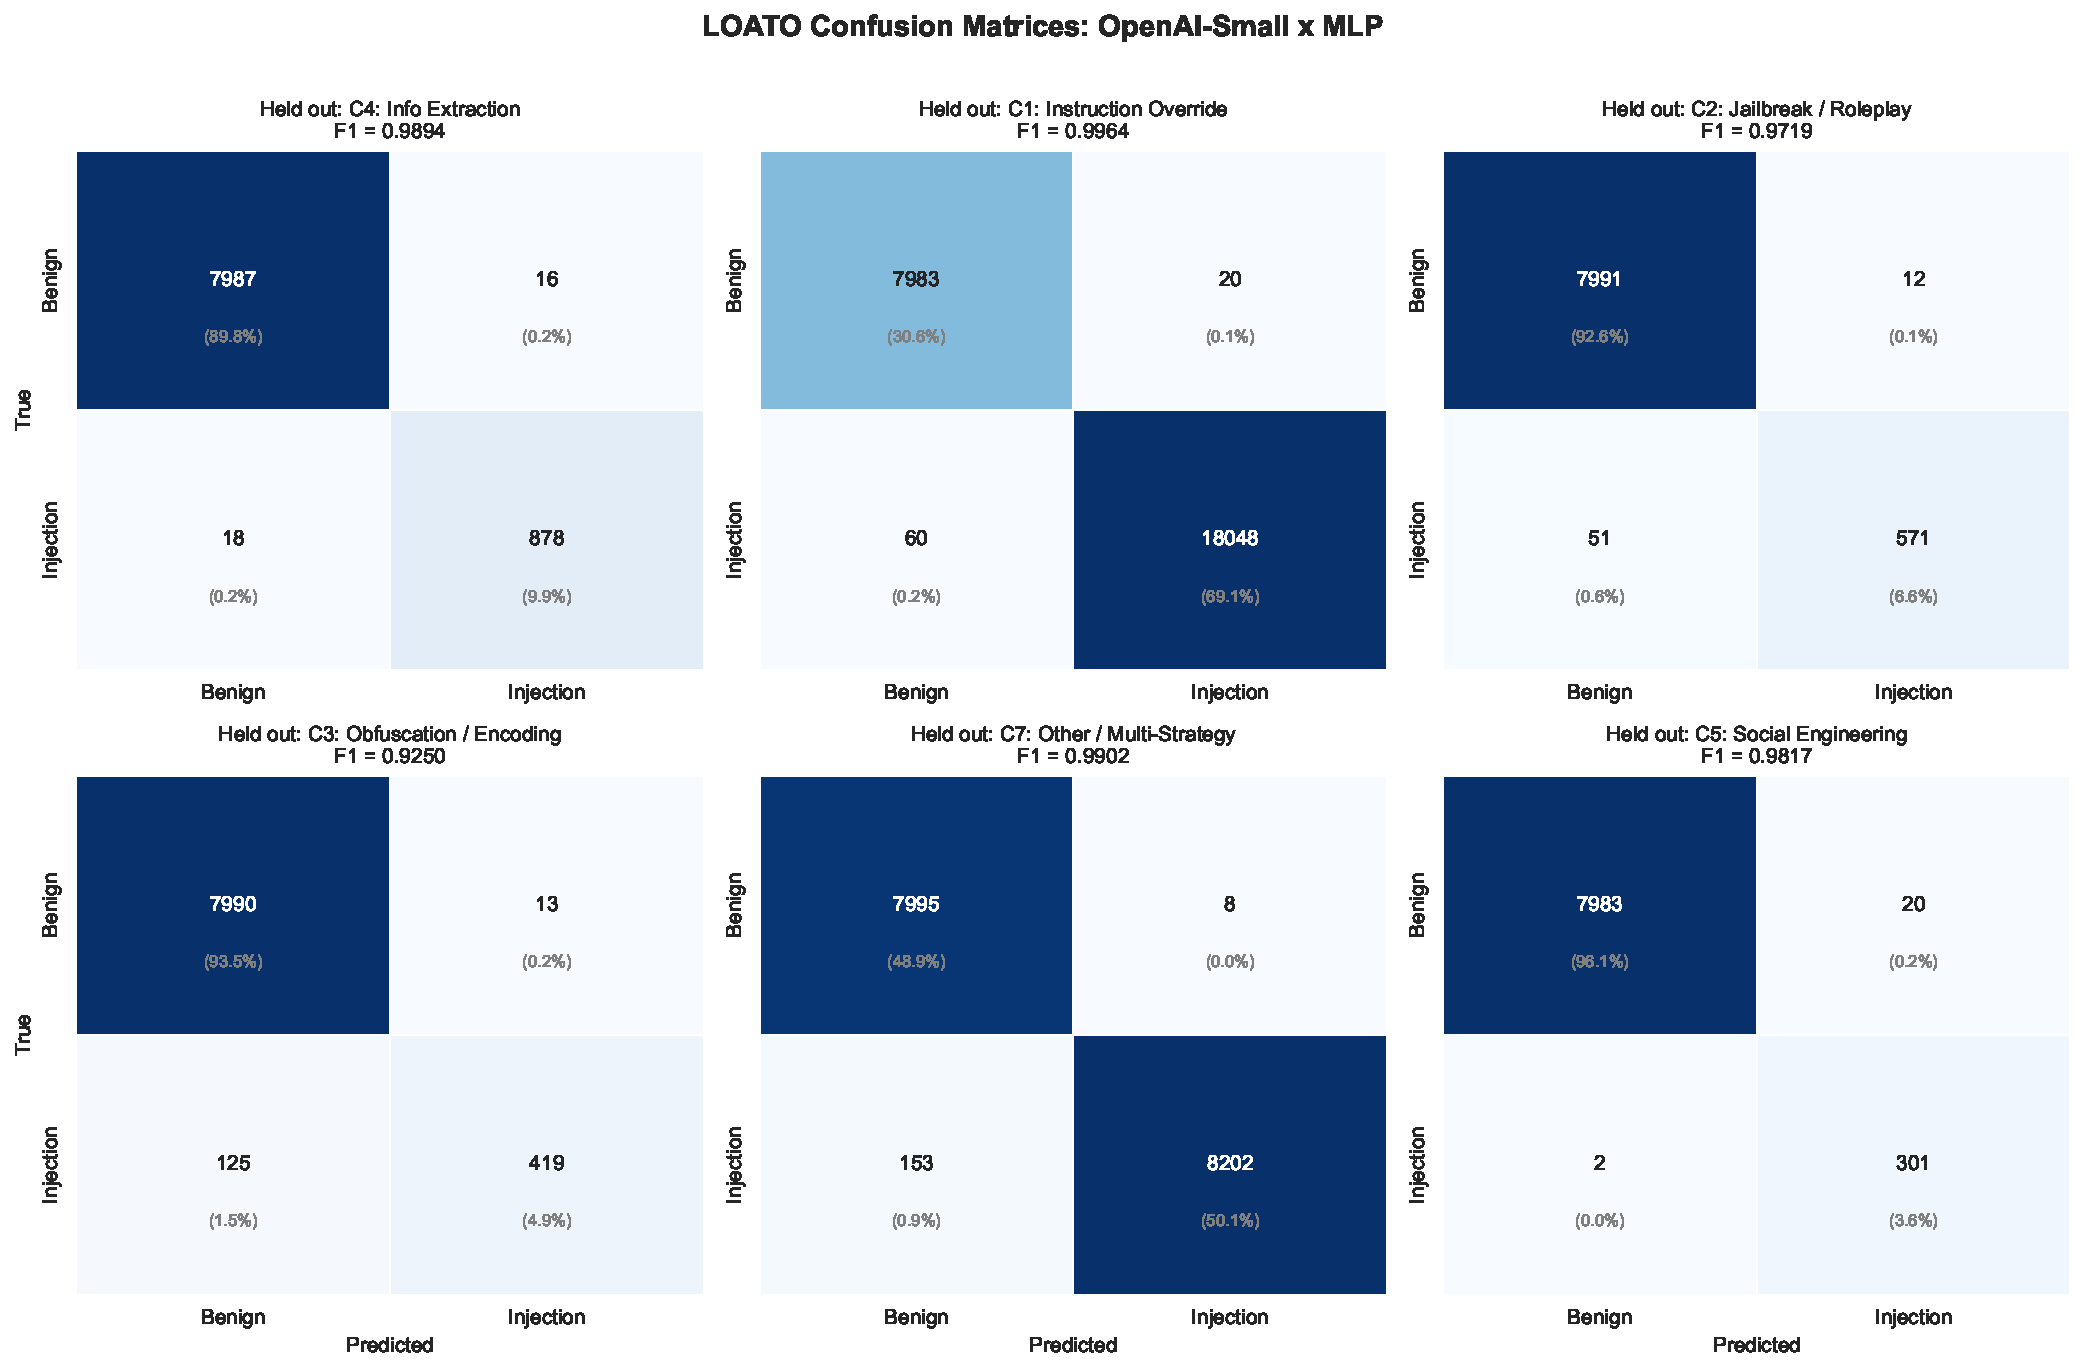
\includegraphics[width=0.85\textwidth]{figures/confusion_matrices_openai_small_mlp.pdf}
  \caption{LOATO confusion matrices for OpenAI-Small $\times$ MLP (best
    overall). Each subplot holds out one attack category. The model maintains
    high true-positive rates across all folds; C3 (Obfuscation) shows the
    most false negatives, consistent with its largest \df{}.}
  \label{fig:cm}
\end{figure*}

\subsection{Direct$\to$Indirect Transfer Collapse}
\label{sec:transfer}

\Fone{} collapses from 0.83--0.97 (standard CV) to 0.21--0.52 on indirect
injections (Table~\ref{tab:transfer}). A classifier that appears 97\% effective
catches only 21--41\% of indirect attacks.

\begin{table}[t]
\centering
\footnotesize
\caption{Direct$\to$Indirect transfer: Macro \Fone{} and AUC-ROC. SVM uses
  Nystroem approximation.}
\label{tab:transfer}
\begin{tabular}{lcccc}
\toprule
& \multicolumn{2}{c}{\textbf{Macro \Fone{}}} & \multicolumn{2}{c}{\textbf{AUC-ROC}} \\
\cmidrule(lr){2-3} \cmidrule(lr){4-5}
\textbf{Embedding} & \textbf{Best} & \textbf{Worst} & \textbf{Best} & \textbf{Worst} \\
\midrule
MiniLM & .290 & .221 & .875 & .816 \\
BGE-Large & .271 & .207$^\dagger$ & .875 & .735 \\
Instructor & .523$^\dagger$ & .226 & .964 & .923 \\
OpenAI-Small & .413 & .218$^\dagger$ & .951 & .871 \\
E5-Mistral & .325 & .206$^\dagger$ & .861 & .684 \\
\bottomrule
\multicolumn{5}{l}{\footnotesize $^\dagger$SVM (Nystroem approx.).}
\end{tabular}
\end{table}

\textbf{AUC-ROC $\gg$ \Fone{}}: classifiers partially \emph{rank} indirect
injections correctly (AUC 0.68--0.96) but decision thresholds calibrated on
direct injections are wrong for the shifted distribution. Threshold
recalibration improves mean \Fone{} from 0.29 to 0.56 (oracle thresholds), but
this still falls far below in-distribution performance (0.96). Most oracle
thresholds require $t \leq 0.01$, which would raise false positives
unacceptably. Threshold tuning is a partial mitigation, not a fix.

\subsection{LLM Zero-Shot Baseline}

GPT-4o evaluated zero-shot on 500 samples per test pool:

\begin{table}[t]
\centering
\footnotesize
\caption{Classifier vs.\ GPT-4o zero-shot comparison.}
\label{tab:llm}
\begin{tabular}{llccc}
\toprule
\textbf{Test Pool} & \textbf{System} & \textbf{\Fone{}} & \textbf{Win} & \textbf{Gap} \\
\midrule
\multirow{2}{*}{Std.\ CV}
  & Best Clf. & .997 & \multirow{2}{*}{Clf.} & \multirow{2}{*}{+.14} \\
  & GPT-4o & .853 & & \\
\midrule
\multirow{3}{*}{\shortstack[l]{Dir.$\to$\\Indir.}}
  & Best non-SVM & .413 & \multirow{3}{*}{GPT-4o} & +.30 \\
  & Best overall$^\dagger$ & .523 & & +.19 \\
  & GPT-4o & .711 & & --- \\
\bottomrule
\multicolumn{5}{l}{\footnotesize $^\dagger$Instr.$\times$SVM (Nystroem).}
\end{tabular}
\end{table}

On familiar attacks, classifiers win (+0.14 \Fone{}, $\sim$800$\times$
cheaper). On novel attacks, GPT-4o wins by +0.30 over the best non-SVM
classifier and +0.19 over the SVM outlier. The gap is architectural:
classifiers drop 0.45--0.56 \Fone{} from standard to indirect; GPT-4o drops
0.14. GPT-4o's precision is near-perfect (0.97--0.99) but recall is limited
(0.63--0.70), making it a reliable second opinion but not a standalone solution.

\subsection{Cost-Performance Analysis}

A layered defense uses the classifier as a first layer with LLM escalation for
uncertain cases (Fig.~\ref{fig:regime}).

\begin{figure}[t]
  \centering
  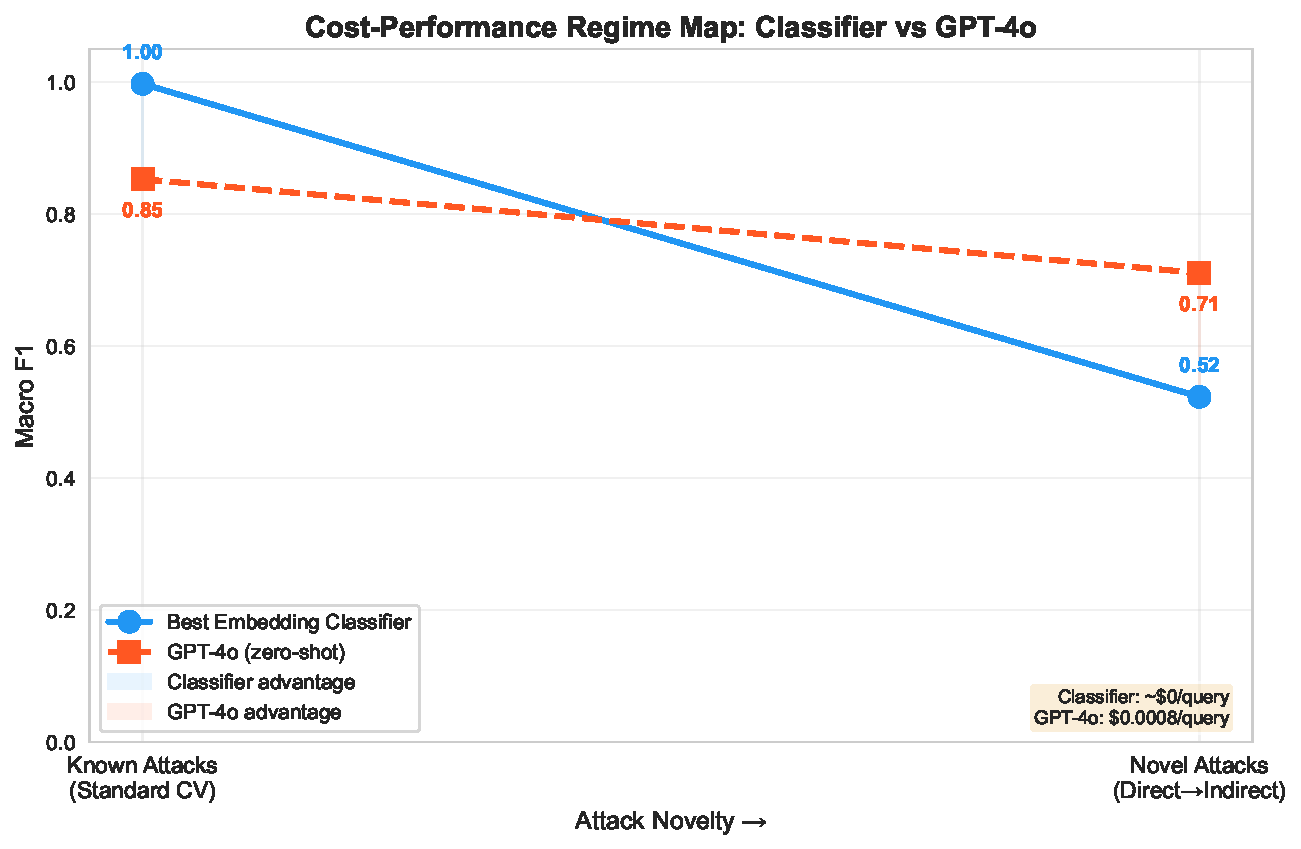
\includegraphics[width=0.95\columnwidth]{figures/cost_performance_regime_map.pdf}
  \caption{Cost-performance regime map: classifier vs.\ GPT-4o on known and
    novel attack surfaces.}
  \label{fig:regime}
\end{figure}

At 10\% escalation, cost is \$0.08/1K queries (80$\times$ cheaper than
GPT-4o-only) with +0.019 \Fone{} gain on novel attacks. At 25\%, cost is
\$0.21/1K (4$\times$ cheaper) with +0.05 \Fone{} gain. GPT-4o's near-perfect
precision (0.99) makes it ideal as an escalation layer---very few false alarms
when it does fire.

% =============================================================================
% 6. DISCUSSION
% =============================================================================
\section{Discussion}
\label{sec:discussion}

\paragraph{Standard CV is misleading.}
A classifier scoring 0.97 \Fone{} under standard CV may score 0.21 on indirect
injections. This is not a minor degradation---it is near-total failure. Standard
CV should not be the sole evaluation for production classifiers.

\paragraph{The failure is architectural.}
Embedding classifiers learn surface patterns. When intent is expressed
differently---embedded in documents, encoded in Base64, delivered through social
engineering---the patterns fail. GPT-4o's zero-shot performance (0.71 \Fone{})
confirms reasoning about intent transfers where pattern matching cannot.

\paragraph{Not all attack types are equally hard.}
LOATO per-fold analysis reveals that some categories generalize well (C1:
Instruction Override, \df{} = 0.037) while others cause large drops (C3:
Obfuscation, \df{} = 0.090). Template homogeneity analysis
(Section~\ref{sec:homogeneity}) shows this correlates with structural similarity
to training categories ($r = -0.742$, $R^2 = 0.550$).

\paragraph{Practical recommendations.}
\begin{enumerate}[nosep,leftmargin=*]
\item \textbf{Evaluate with LOATO} before deploying. Report per-category
  \Fone{}, not just aggregate. Flag any category with \df{} $> 0.15$.
\item \textbf{Test direct$\to$indirect transfer} for RAG/tool-use deployments.
  Standard CV is not predictive.
\item \textbf{Use layered defense}: classifier first layer ($\sim$\$0/query),
  LLM escalation for uncertain cases. At 10\% escalation, 80$\times$ cheaper
  than LLM-only with modest \Fone{} loss.
\item \textbf{Threshold calibration is a band-aid}: improves transfer \Fone{}
  from 0.29 to 0.56 on average, but remains far below in-distribution
  performance (0.96).
\end{enumerate}

% =============================================================================
% 7. LIMITATIONS
% =============================================================================
\section{Limitations}
\label{sec:limitations}

\begin{enumerate}[nosep,leftmargin=*]
\item \textbf{C6 excluded from LOATO}---only 188 samples, 12 short of the 200
  threshold. This is the most deployment-relevant category; its
  underrepresentation in public datasets is itself a finding.
\item \textbf{English-only}---98\% of samples are English. Cross-lingual
  experiments were excluded ($<$300 samples per language).
\item \textbf{Single LLM baseline}---only GPT-4o evaluated. Additional models
  would strengthen generality claims.
\item \textbf{SVM uses kernel approximation}---Nystroem(500) + PCA(128) for
  tractability. SVM results are a lower bound on exact-kernel performance.
\item \textbf{Low statistical power for LOATO gaps}---only 3/20 are significant
  ($p < 0.05$) with 5--6 folds. Gaps are consistently positive but most
  $p$-values fall in 0.06--0.15.
\end{enumerate}

% =============================================================================
% 8. CONCLUSION
% =============================================================================
\section{Conclusion}
\label{sec:conclusion}

Embedding-based prompt injection classifiers achieve 0.977--0.997 \Fone{} under
standard CV, but LOATO reveals a mean \df{} = 0.051 with category-dependent
blind spots, and direct-to-indirect transfer shows \Fone{} collapsing to
0.21--0.41. GPT-4o achieves 0.71 \Fone{} zero-shot on the same indirect test
set, a +0.30 advantage at $\sim$800$\times$ higher cost. We recommend
LOATO-style evaluation as standard practice, layered defenses combining cheap
classifiers with LLM escalation, and explicit transfer testing for any system
processing untrusted content. Standard CV scores are reassuring. The real world
is not.

% =============================================================================
% REFERENCES
% =============================================================================
\bibliographystyle{IEEEtran}
\bibliography{references}

% =============================================================================
% APPENDIX
% =============================================================================
\appendix

\section{Reproducibility}
\label{app:repro}

{\small
\begin{verbatim}
uv sync                          # Environment
uv run loato-bench data download # Data pipeline
uv run loato-bench data harmonize
uv run loato-bench data label
uv run loato-bench data split
uv run loato-bench embed run --all  # Embeddings
uv run loato-bench train run --all \
    --experiment standard_cv --wandb
uv run loato-bench train run --all \
    --experiment loato --wandb
uv run loato-bench train run --all \
    --experiment direct_indirect --wandb
uv run loato-bench analyze llm-baseline \
    --model gpt-4o --samples 500
uv run loato-bench analyze report
\end{verbatim}
}

\noindent Requirements: Python 3.12, \texttt{uv}, HuggingFace token, OpenAI API
key. Seed: 42. Hardware: Apple Silicon Mac (18~GB).

\section{Full Results}
\label{app:full-results}

\begin{table}[h]
\centering
\footnotesize
\caption{Mean LOATO \Fone{} by held-out category (averaged across all 20
  embedding-classifier combinations). Full per-combo breakdown available
  in the project repository.}
\label{tab:per-fold-summary}
\label{tab:full-results}
\begin{tabular}{llcc}
\toprule
\textbf{Held-Out} & \textbf{\Fone{}} & \textbf{Hardest} & \textbf{Easiest} \\
\midrule
C7 Other & .951 & BGE$\times$SVM & BGE$\times$MLP \\
C1 Instr.\ Ovr.\ & .946 & E5$\times$SVM & Instr.$\times$MLP \\
C4 Info.\ Extr.\ & .926 & Instr.$\times$SVM & OpenAI$\times$MLP \\
C2 Jailbreak & .919 & Instr.$\times$SVM & OpenAI$\times$MLP \\
C5 Social Eng.\ & .910 & BGE$\times$SVM & E5$\times$MLP \\
C3 Obfusc.\ & \textbf{.874} & Instr.$\times$SVM & BGE$\times$MLP \\
\bottomrule
\end{tabular}
\end{table}

\end{document}
